\documentclass[a4paper,UKenglish]{article}
\usepackage[utf8]{inputenc}
\usepackage{fontenc,url}
\usepackage{babel,textcomp}
\usepackage[round]{natbib}
\usepackage{graphicx}
\usepackage{subcaption}
\graphicspath{ {images/} }
%\urlstyle{sf}

\title{Report1}
\author{Kasper Skjegggestad}
\begin{document}
\maketitle
\tableofcontents

\section{Introduction}

\section{Goal}

The goal of this study is to generate a DTM from ASTER stereo imagese, orthorectify it, and assess accuracy of the DTM. The DTM and the ortophoto will be compared to DTM from Statens Kartvært and DTM generatet from silcAst. 

\section{ASTER DEM production}

The DEM var generated with ASTER stereo image data Level 1B in Geomatica of PCI. The first object, after loading the image into the software, was to collect Global Controll Points (GCPs). On the NADIR image, reconaceble places in the map was found, mostly the pointed ends of lakes. The elevation and cooridnates for the points was gatherd from a DEM and maps from Kartverket. Kartværket had a tile map consisting of 9 tiles over the area of intrest. Each tile was used to ensure GCPs over the entire aeria. The points was then transfered to the backlooking image. Most GCPs had to be adjusted to represent the same point. Approximately 30 points was found althogheter, but some of the points was outside the aeria of the backlooking image. Therese points was therfore put to check in the backlooking image, so not to affect the DEM. Tie-points was then collected. PCI geomatica did this automaticly for me.

Next i created an Epipolar image with 3N and 3B, now i can extract DEM. In the interface of 'Extract DEM automatically', I let most of the parameters stay on default, but change the terring to mountinus.

\section{Orthoprojection}

The 'Ortho Generation' step in PCI was done with both 3N and 3B and with my own DEM and Statens Kartverk DEM.

\section{Analysis}

\begin{figure}
	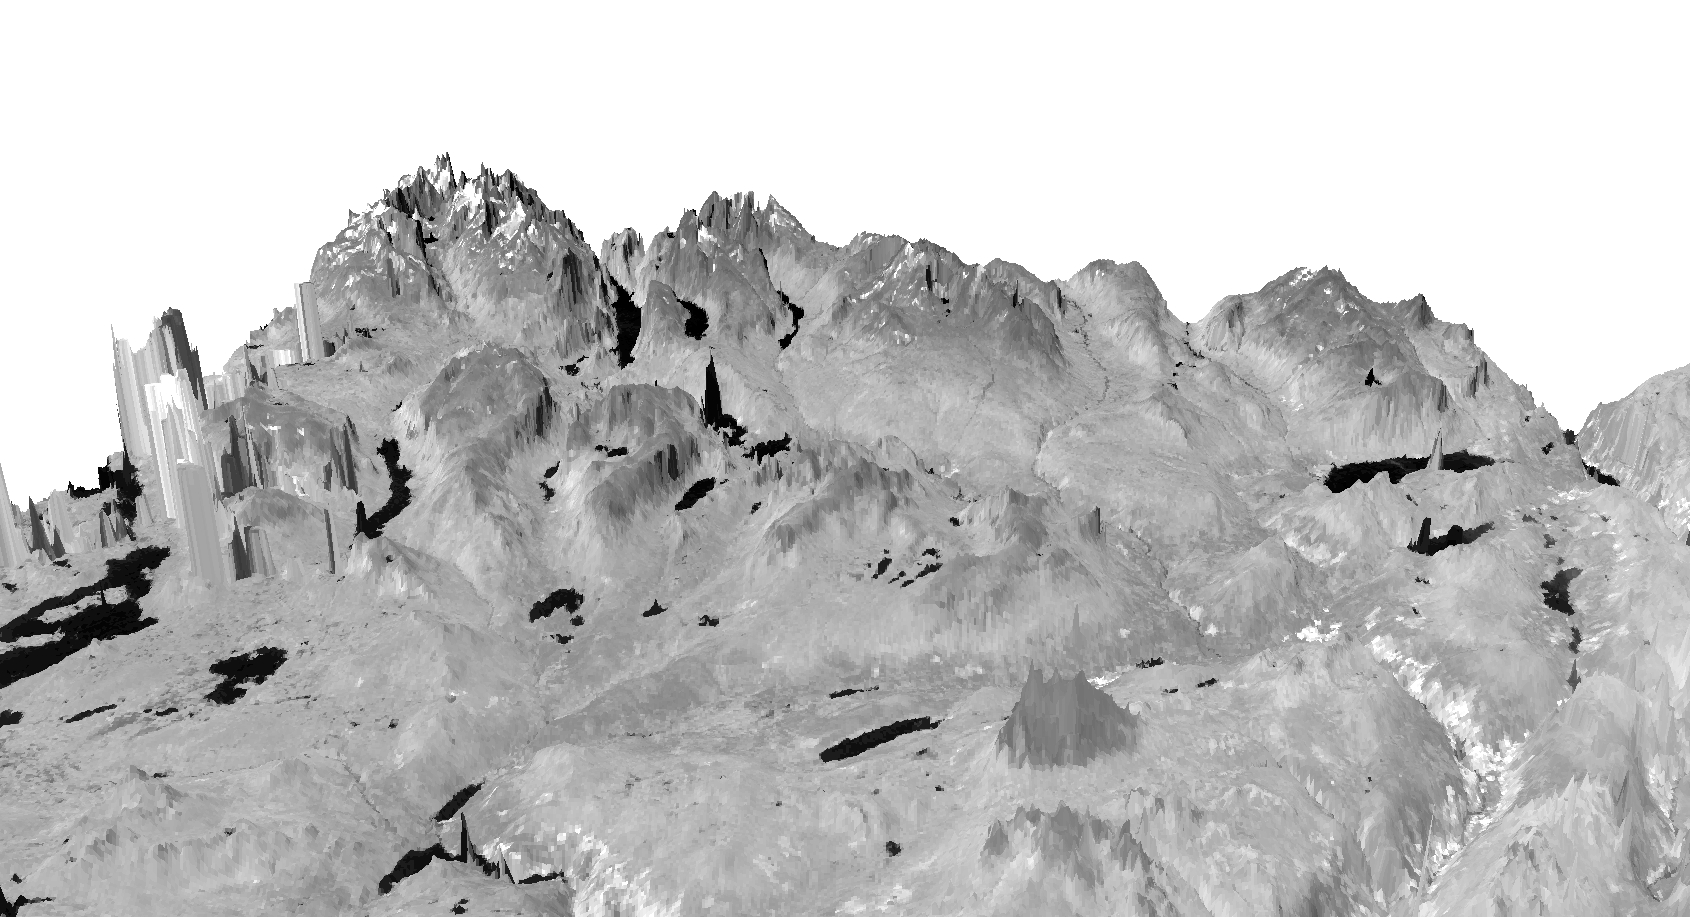
\includegraphics[height=8cm]{3dbilde2}
	\caption{3D representation of new DEM over ortopotho}
	\label{3dimage}
\end{figure}

In the newly generated DTM, there are some clear outliers. Therese can easly be seen in a 3D representation of the DEM (figure \ref{3dimage}). On the left of figure \ref{3dimage}, there are some really high, steep "mounteins". This is cloudes from the stellitte image. The clouds are blocking the satellittes view of the ground terrein, and we will therefor not get reliable data in therese aeraias. A little left of the center in figure \ref{3dimage}, and to the right in the figure, tall black "mountains" can be spottet. Therese are located in lakes, and therfor there can not be any mouintan here and are therfor errors in the DEM. When adding countour lines over the ortophotho, some more erros are spottet. The small hills in the lakes, that clearly should not be there, are spottet, as well as massive gathering of countoiurlines around the coulds.

\begin{figure}
	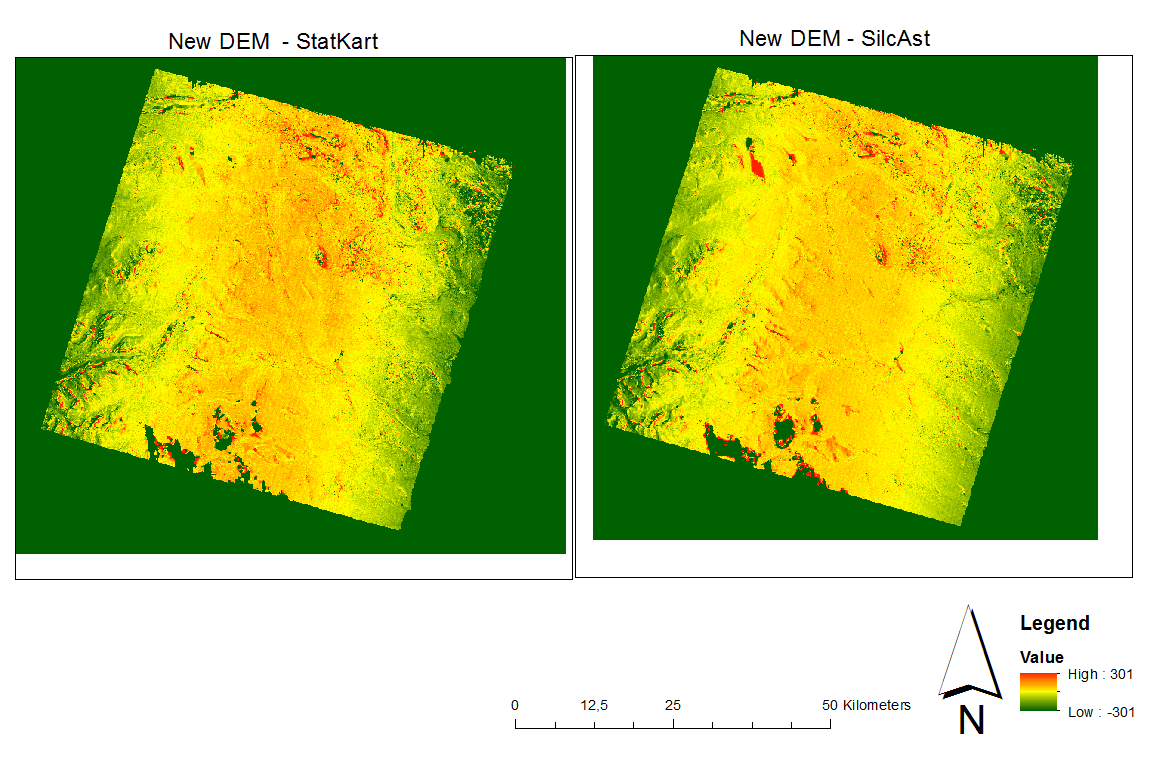
\includegraphics[height=8cm]{DiffJotun-StatogSil}
	\caption{The Different between the new DEM of Jotunheimen and the DEM of statkart and from silcAst of Jotunheimen}
\end{figure}

\begin{figure}
	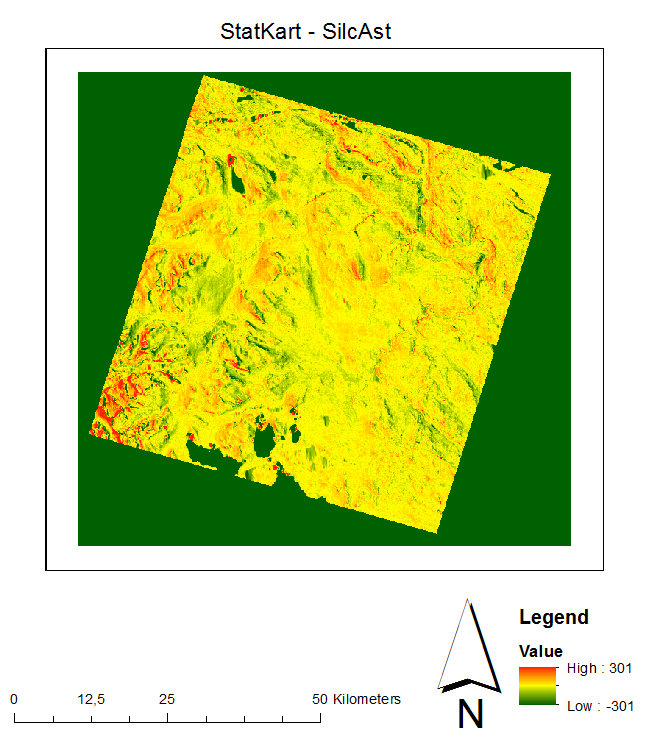
\includegraphics[height=8cm]{DiffJotun-Stat-Sil}
	\caption{The difference between the DEM of Jotunhemien from statkart and silcAst}
\end{figure}

When calculating the difference beween the newly generated ASTER DEM, a DEM generated of silcast and karverkets DEM, it is reviled that the new DEM has larger errors in the south east and north west periferi. This systematic error is not precent when we look at the different between silcast and karverket, indicating that this error in the newly generated DEM onely.

Probably because of the coulds, there are big outliers between the DEMs. Yo cut out some of the out liers, the Standar derivaton (Std) is used. All absolute values above 3 times the Std will be set to NaN values (Not a Number). This reduses the RMSE and the new Std with more than 50$\%$. The median of the differance hardly changes, while the mean shows significant changes in most  plots. 


\begin{figure}
	\begin{subfigure}{.5\textwidth}
		  \centering
		  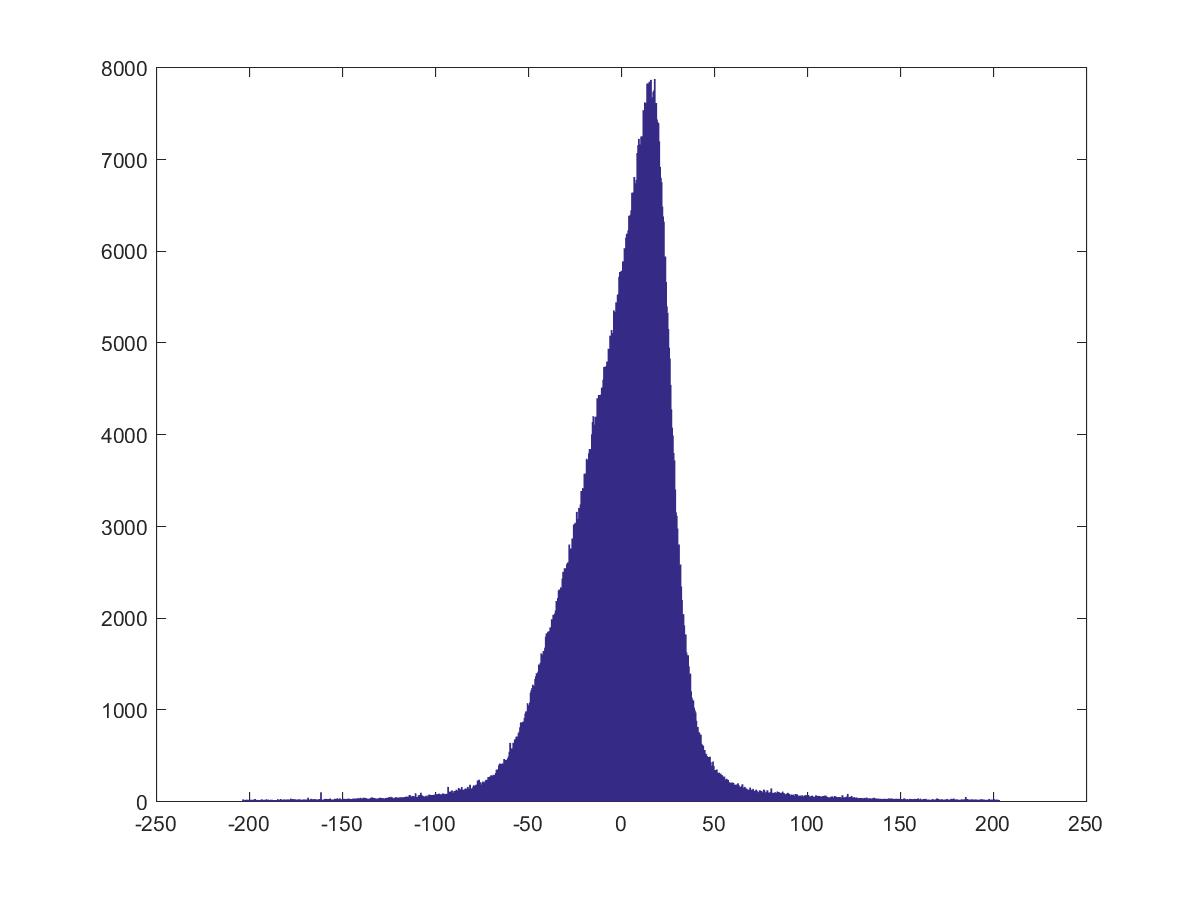
\includegraphics[width=.8\linewidth]{hist_SJD}
		  \caption{New DEM - StatKart DEM}
		  \label{fig:sfig1}
	\end{subfigure}%
	\begin{subfigure}{.5\textwidth}
		  \centering
		  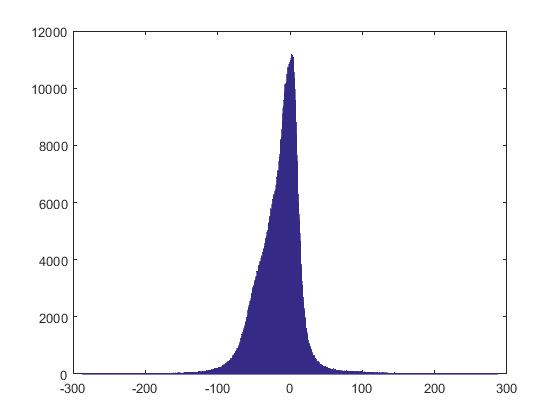
\includegraphics[width=.8\linewidth]{hist_SiJD}
		  \caption{New DEM - SilcAst DEM}
		  \label{fig:sfig2}
	\end{subfigure}
	\begin{subfigure}{.5\textwidth}
	  \centering
	  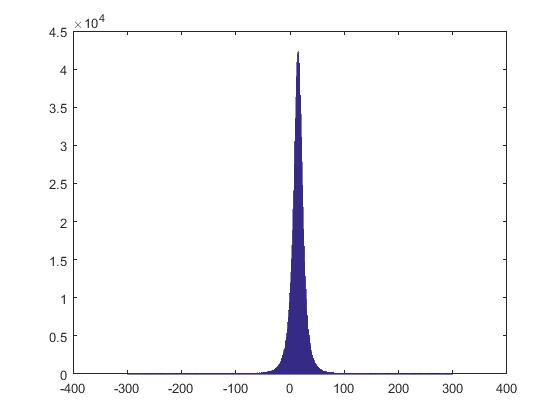
\includegraphics[width=.8\linewidth]{hist_SSiD}
	  \caption{StatKart DEM - SilcAst DEM}
	  \label{fig:sfig3}
	\end{subfigure}
		\caption{A histogram of the values in the all the DEM differances of Jotunheimen}
		\label{fig:fig}
\end{figure}


\section{Conclution}

\end{document}
